\section{Introduction}\label{setion:introductionMyBioMecaModel}
State of the art in breast finite elements modeling was described previously. Three model were identified representing the cutting-edge  technologies in the field. These models use prone MRI to create the breast reference geometry and supine MRI to compute patient-specific tissues mechanical properties. The models were evaluated using  the measured and the estimated position of the superficial fiducial landmarks or internal anatomical landmarks in supine configuration.   However, the authors assumed different boundary conditions and considered different tissues types.  
In addition, none of the previous works have quantitatively evaluated the proposed model on an additional data set of the same patient. 

 This chapter present a new biomechanical model developed by combining the best practices and concepts proved by previous works. To be as realistic as possible, our model considered breast heterogeneity, anisotropy, sliding boundary conditions, initial pre-stresses and personalized hyper-elastic properties of breast tissue. In addition, new types of soft tissue were included representing the breast support matrix composed of suspensory ligaments and fascias. Moreover, our model was built using prone and supine breast configurations and was evaluated in supine tilted configuration (~ 45 degrees) of the same volunteer.

In the first part of this chapter the data acquisition protocol is described and details on numerical methods and softwares used to extract the patient specific breast geometry are given. Next, the different components of the finite elements mesh are presented and the mesh quality is assessed using shape parameters.  Then, the assumptions on boundary condition and materials models are explained. Finally the model optimization process is detailed and results on patient specific parameters and breast reference configuration are presented.   
\clearpage
\section{Geometry extraction}\label{section:geometryextraction}

Geometry extraction is the first step in FE analysis, and it
consists of obtaining the 3D surface of the
breast. We use the MR images to obtain the patient-specific breast volumes and the surrounding soft tissues distribution. Prior to surface extraction the MRI volume is segmented and mapped to a single reference system. The next section describe the imaging acquisition protocol and the numerical method used to generate the 3D patient specific breast geometry.

\subsection{Data acquisition}%\label{subsection:imageaquisition}

 The images were acquired with a Siemens 3T scanner with T2 weighted image sequences. The in-plane image resolution was $0.5$x$0.5$ mm, and the slice thickness was 0.6 mm. During this acquisition, the contact between the breasts and the contours of the MRI tube, or with the patient body (arms, thorax), was minimized.
\begin{figure}[H]
\centering
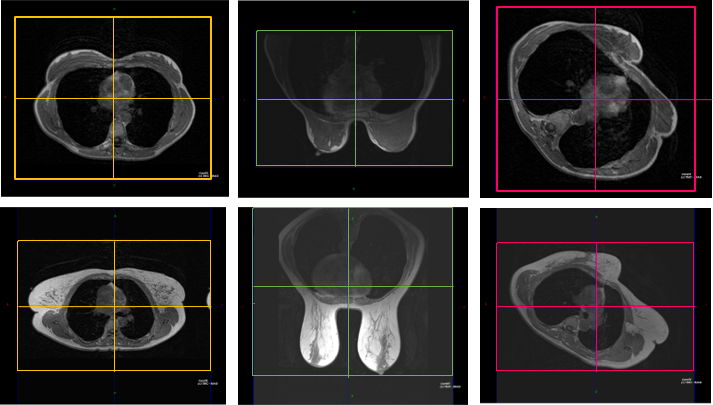
\includegraphics[width=0.9\textwidth,keepaspectratio]{figures/patientData.png} 
\caption{MRI images in three breast configuration: first line- subject 1; second line- subject 2}\label{fig:patientdata}
\end{figure}

The two volunteers taking part to this study agreed to participate in an experiment part of a pilot study approved by an ethical committee (MammoBio MAP-VS pilot study). The volunteers are 59 and 58 years old and have A-cup (subject 1) and F-cup (subject 2) breast size respectively. 

Three different positioning configurations are considered: prone, supine and supine titled (\~ 45 deg). The positions were chosen to assess the largest possible deformations with minimal contact areas between the volunteer and the relatively narrow MRI scanner tunnel. 

The volunteers were also asked to provide the compression force and breast thickness as measured on their most recent mammograms. Such data are summarized in Table \ref{tab:forceandthichnessdata}.
\begin{table}[H]
\centering
\begin{tabular}{c|c|c||c|c|}
\cline{2-5}
&\multicolumn{2}{c||}{Subject 1}&\multicolumn{2}{c|}{Subject 2}\\
\cline{2-5}
& Right breast & Left breast & Right breast & Left breast\\
\cline{2-5}
\hline
\multicolumn{1}{|c||}{Force (N)}  & 21.9 &40.9 &94.8 & 56.6 \\
\hline
\multicolumn{1}{|c||}{ Breast thickness (mm)} & 47 & 42 & 50 & 49 \\
\hline

\end{tabular}
\caption{Compression force and breast thickness for both subjects for a cranio-caudal mammogram}\label{tab:forceandthichnessdata}
\end{table}


\subsection{Image segmentation}%\label{subsection:imagesegmentation}

A semi-automated active contour method proposed by ITK-Snap software is used to segment the pectoral muscle, the breast and the internal organs from MR images. 

The segmentation process for one tissue type is performed progressively by small regions of interest (ROI, see Figure \ref{fig:breasttissuessegmentation}.a). For each ROI the segmentation of one tissue takes place in 3 steps (Figure \ref{fig:breasttissuessegmentation}):
\begin{enumerate}
\item Firstly, the random forest algorithm is used to compute the probability of a pixel to belong or not to the segmented tissue. The training data is manually selected by the user and include state and space characteristics as: voxel grey intensity, voxel's neighbors intensity (with variable radius of neighboring), (x; y; z) voxel position (Figure \ref{fig:breasttissuessegmentation}.c ).

\item Secondly, spherical seeds point with variable radius are placed on the new synthetic volume to mark the connected components bellowing to the segmented tissue (Figure \ref{fig:breasttissuessegmentation}.d).
\item Finally, the placed seed point will evolve in the 3D space with a speed and direction derived from the pixel intensity and sign in the synthetic volume (Figure \ref{fig:breasttissuessegmentation}.d).
\end{enumerate}

 
 \begin{figure}[H]
\centering
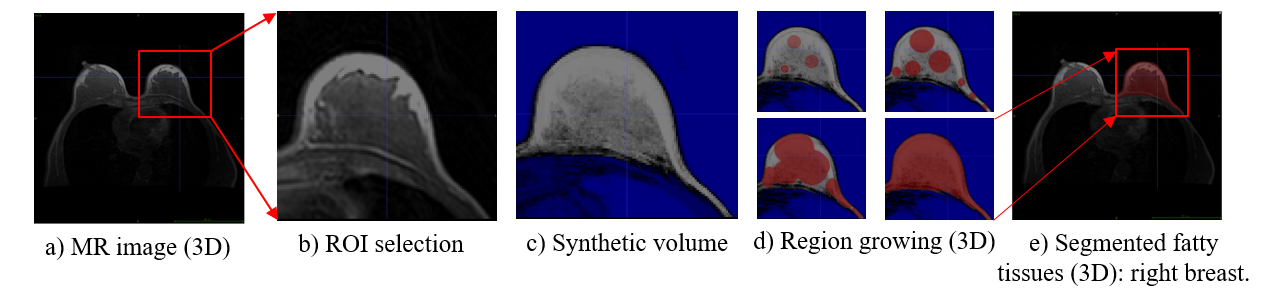
\includegraphics[width=1\textwidth,keepaspectratio]{figures/tissues_segmentation.png} 
\caption{Breast tissues segmentation on the breast MRI of the second subject. Prone breast configuration. White-voxel belongs to breast tissue; blue - voxel don't belongs to fatty tissue} \label{fig:breasttissuessegmentation}
\end{figure}

 After segmentation, an additional manual correction was performed to refine components boundaries. Simple erosion and dilatation operations were applied on breast and muscle segmented volumes in order to obtain smoother connected components. Then, to avoid tissues overlapping at muscle-breast juncture border binary operations were used.
 
The process was repeated for both volunteers and for each breast configuration: supine, prone and supine tilted.

\subsection{Image registration}\label{subsection:image registration}

During the imaging acquisition process, the subject is moved in and out the MRI scanner. Therefore, the breast not only undergoes an elastic transformation, but also a rigid one. Prior to image acquisition, four landmarks are fixed on the chest wall.  The landmarks are placed on sternum and inframammary fold lines; regions known to be rich in fibrous ligaments limiting the soft tissues elastic deformation.  To assess the body position changes between the two configurations a rigid transform is computed by minimizing the Euclidian distance of the four points defined by the four landmarks. The transformation is estimated using the iterative closest point (ICP) algorithm proposed by ITK library.

However, because of breast hyperelasticity the computed transformation is not accurate enough. Therefore, a second registration step is performed by aligning the bone structures of the anterior part of thoracic cage from prone and supine tilted positions to the supine one. The muscular tissues mask previously segmented are used in order to remove body soft tissues. The image registration is implemented using the descendant gradient based algorithm minimizing the images cross correlation (ITK library).

Figure \ref{fig:patientdataregistered} shows overlapping  prone-supine and supine tilted-supine breast images in the transversal plane after registration. The anterior part of the chest line is wall aligned, however there are some differences because of elastic thoracic cage deformation due to hand positions or body-mass force reparation. 

\begin{figure}[!h]
\centering
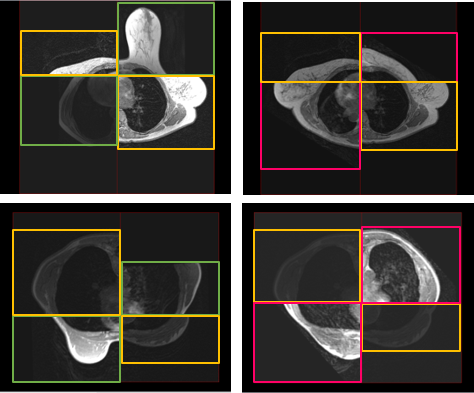
\includegraphics[width=0.7\textwidth,keepaspectratio]{figures/patientDataRegistered.png} 
\caption{Registered MRI images: first line- subject 1; second line- subject 2; first column - prone configuration versus supine; second column - supine tilted versus supine }\label{fig:patientdataregistered}
\end{figure}

In a  multy-gravity loading finite elements simulation, the gravity force is applied to the whole model as a body force. The gravity fore orientation can be broken down into three components of the Cartesian coordinate system labeled X, Y, and Z directions. The supine configuration was chosen as a reference state, therefore the gravity loading direction was set to be oriented on the inverse direction  of the Z axis (posterio-anterior direction): $\gamma_s = (0,-1,0)$.   The gravity loading direction for the two other positions are given by the rigid transformation computed by images registration: $\gamma_p = (0.037, 0.985, -0.165)$ direction vector for gravity in prone position and $\gamma_{st} = (-0.744 , -0.667, 0.023)$ direction vector for supine tilted position.

\begin{figure}[!ht]
\centering
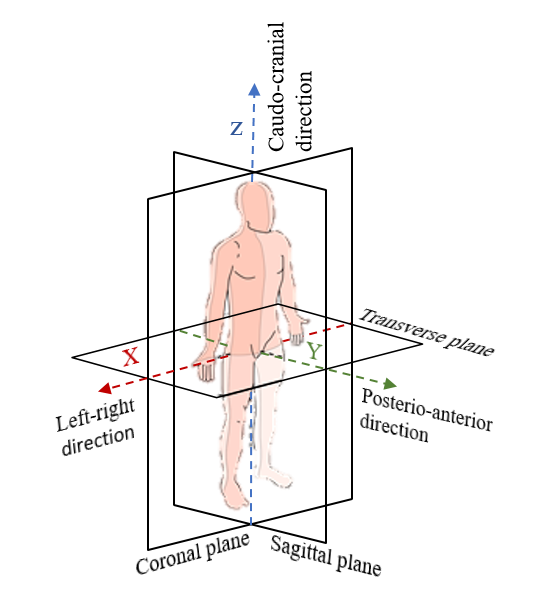
\includegraphics[width=0.7\textwidth,keepaspectratio]{figures/xyz_axis_directions.png} 
\caption{Anatomical planes and nominal Cartesian axis directions.}\label{fig:xyz_axis_directions}
\end{figure}

\subsection{Patient-specific 3D geometry}

\label{subsection:patientspecificgeometry}

The breast patient-specific geometry was created based on the MR images of the second subject. Following image segmentation (Figure \ref{fig:3dgeometries}.b), the outer shape of labeled regions are subsequently discretized by 2D triangular elements.  We used the semi-automatic Skin Surface module proposed by SpaceClaim Direct Modeler to convert the mesh surfaces to non-uniform rational basis spline (NURBS) surfaces. The NURBS are averaging curves between points, therefore they are smoother and easier to use in mechanical applications. The resulting  two surface represent the 3D geometries of the breast and the thoracic cage with muscle  (Figure \ref{fig:3dgeometries}.c).   
 

\begin{figure}[!h]
\centering
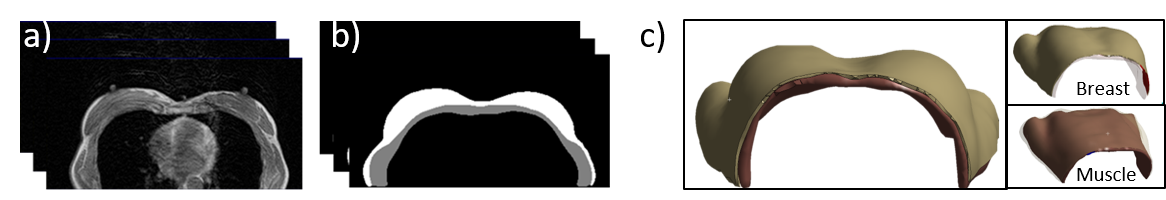
\includegraphics[width=0.9\textwidth,keepaspectratio]{figures/3dgeometries.png} 
\caption{3D geometries generation. a) MR images; b) segmeted image; c) corresponding 3D geometries}\label{fig:3dgeometries}
\end{figure}

\section{ Finite Elements Mesh}\label{section:myFEM}

After computing the NURBS surfaces, the internal spatial information needs to be encoded using a volumetric mesh. The optimal elements type or mesh density in the simulation of FE models is still an open problem and topic of debate. The use of hexahedral elements results in a more accurate solution, especially when expecting high strain/stress gradients. However, in literature, because of the large computational time, they are used mostly with a reduced number of elements \citep{ruiter_model_based_2006,gamage_modelling_2012}. Tetrahedral elements are widely used due to their geometrical flexibility and because they provide a good trade-off between the computation time and displacement accuracy \citep{han_nonlinear_2014,palomar_finite_2008,griesenauer_breast_2017}.   

In our case, an iterative optimization process is being considered, thus to reduce the computation time  only linear tetrahedral elements are used. The first order elements are known to bear volumetric locking problems when used to model large strain for quasi-incompressible materials, \citep{fung_classical_2017}. Then volumetric locking occurs, the displacements calculated by the finite element method are orders of magnitude smaller than they should be. It have been shown that a linear element with a mixed U-P formulation can avoid these problems \citep{rohan_finite_2014}. In our work, the geometries are meshed using the solid element solid285 (ANSYS Mechanical) which provide a mixed U-P formulation option. 

 On the other hand, the mesh density have also an impact on model accuracy, a finer mesh results in a more accurate and stable solution, but also increase the computational time. So far, no experimental studies have determined the optimal resolution of the volumetric mesh for simulation of breast tissues deformation. To determinate the appropriate mesh size, a mesh convergence study was performed. The details can be found in annex ....  According to these results the optimal element’s sizes range between 7 and 10mm. The chosen mesh consists in 18453 elements with 9625 elements assigned to the pectoral muscle and the toracic cage and 8828 elements assigned to breast tissues (Figure \ref{fig:meshcomponents}).
 
 
 The mesh quality is measured using three criteria: element skewness, aspect ratio and maximal corner angle. The Figure \ref{fig:meshquality} shows the ranges of values for different elements shape parameters. The element's aspect ratio and maximal corner angle range between the nominal limits defining a good mesh quality (Section \ref{section:lagrangianmesh}). There is a small number of elements with a skewness lager than the maximal theoretical quality limit ( 0.75 ) , however there are no degenerated elements (skewness = 1).  

\begin{figure}[!h]
\centering
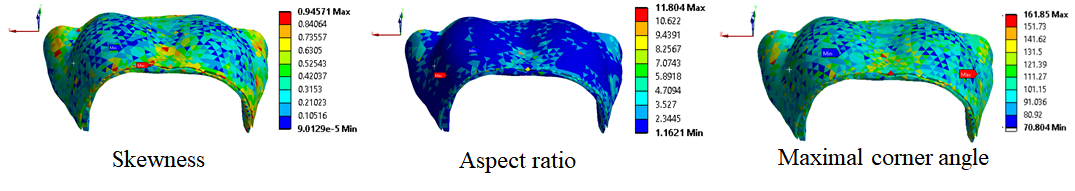
\includegraphics[width=1\textwidth,keepaspectratio]{figures/meshquality.png} 
\caption{Finite elements mesh quality.}\label{fig:meshquality}
\end{figure}


The breast skin layer is added a posteriori   as a $2mm$ thick single layer of shell elements (1980 elements). Shell elements and the underlying solid elements are sharing the same nodes (Figure \ref{fig:meshcomponents}).

\begin{figure}[!h]
\centering
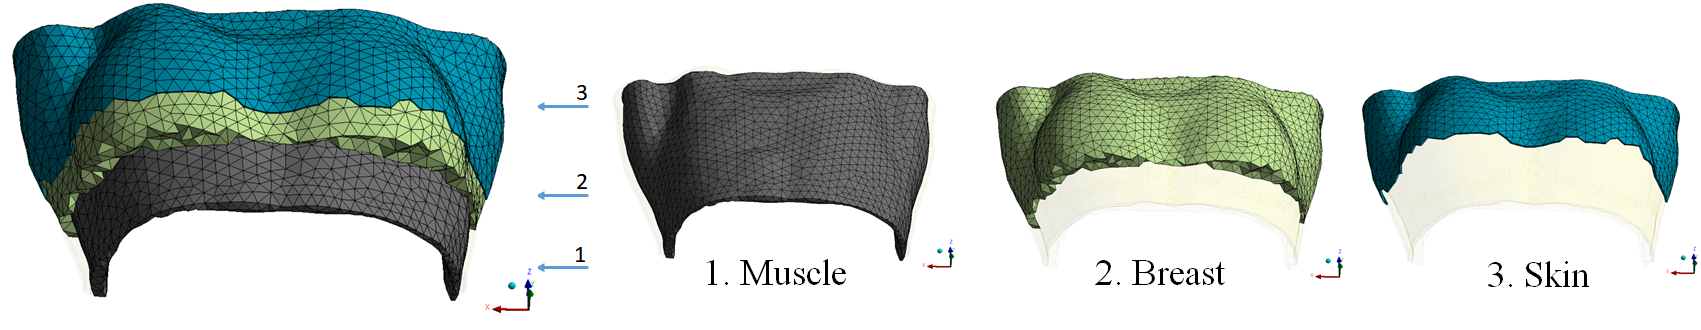
\includegraphics[width=0.9\textwidth,keepaspectratio]{figures/mesh3components.png} 
\caption{Finite elements mesh components. The tissues components are cropped for visualization purposes.}\label{fig:meshcomponents}
\end{figure} 

\section{Breast stress-free geometry}\label{section:myStressFree}
To estimate the stress-free configuration of the breast, an adapted prediction-correction iterative approach was implemented. Prone and supine image data sets are used to compute the stress-free geometry. The overall iterative process is presented in Figure \ref{fig:myfixedpointalgo}. The first estimate of stress-free breast configuration is obtained by inverse gravity on supine geometry. Then, at each iteration, the estimated stress-free configuration is used to simulate breast deformation due to gravity in a prone position. The differences between result of this simulation and the real shape of the breast in prone position is quantified by computing the Euclidian distance $D_i$ between the \textit{active nodes} defined at the breast external surface. This distance is then used in the next iteration of our process to simulate an imposed displacement (Dirichlet condition) to the active node i in the stress-free condition. To limit any mesh distortion, the displacement is only partially imposed using a multiplicative regularization factor $ (\lambda<1)$. The process repeats as long as the new transformation improves the similarity between two geometries by more than $1mm$ on average. The similarity between the estimated and measured prone breast configuration is given by the mean Euclidean distance over the active nodes.                                                              

\begin{figure}[!h]
\centering
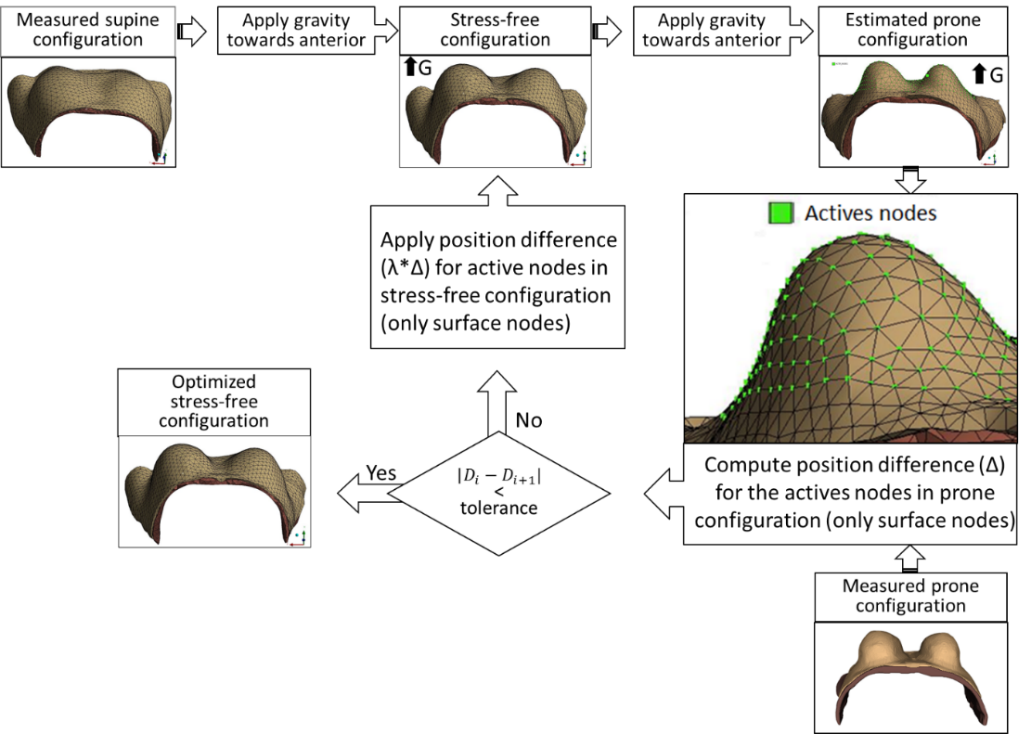
\includegraphics[width=0.9\textwidth,keepaspectratio]{figures/stress_free_config_algo.png} 
\caption{Fixed point type iterative algorithm for stress-free geometry approximation. $D_i$ - mean node to node distance over the active nodes at iteration $i$, $G$ - gravity force}\label{fig:myfixedpointalgo}
\end{figure}

To compute the node-to-node distance $D_i$, the active nodes position on prone configuration have to be known. Thus, an additional mesh registration step is performed at each iteration. The active nodes are morphed into prone configuration using the elastic deformation method proposed by \cite{bucki_fast_2010}. The method estimates a C1-diffeomorphic, non-folding and one-to-one transformation to register a source point cloud onto a target data set D, which can either be a point cloud or a surface mesh.  The input source points set is initially embedded in a deformable virtual hexahedral elastic grid. Then an iterative registration technique is performed by successive elementary grid deformations and at different grid refinement level. 

\section{Boundary conditions}\label{section:myBoundayconditions}

Breast deformation can be modeled by solving the
motion equations using two different types of boundary
conditions, regarding either displacement (Dirichlet conditions) or force (Neumann conditions).

First, to provide a rigid support for the muscle mesh component, zero displacement conditions are imposed to its posterior face  (figure \ref{fig:meshboundaries}). Next, the interface between the breast mesh and muscle mesh is models using contact mechanics. The muscle is stiffer than the adipose tissues, thus it's anterior face represents the target surface and the posterior breast face represents the contact surface. 

\begin{figure}[!h]
\centering
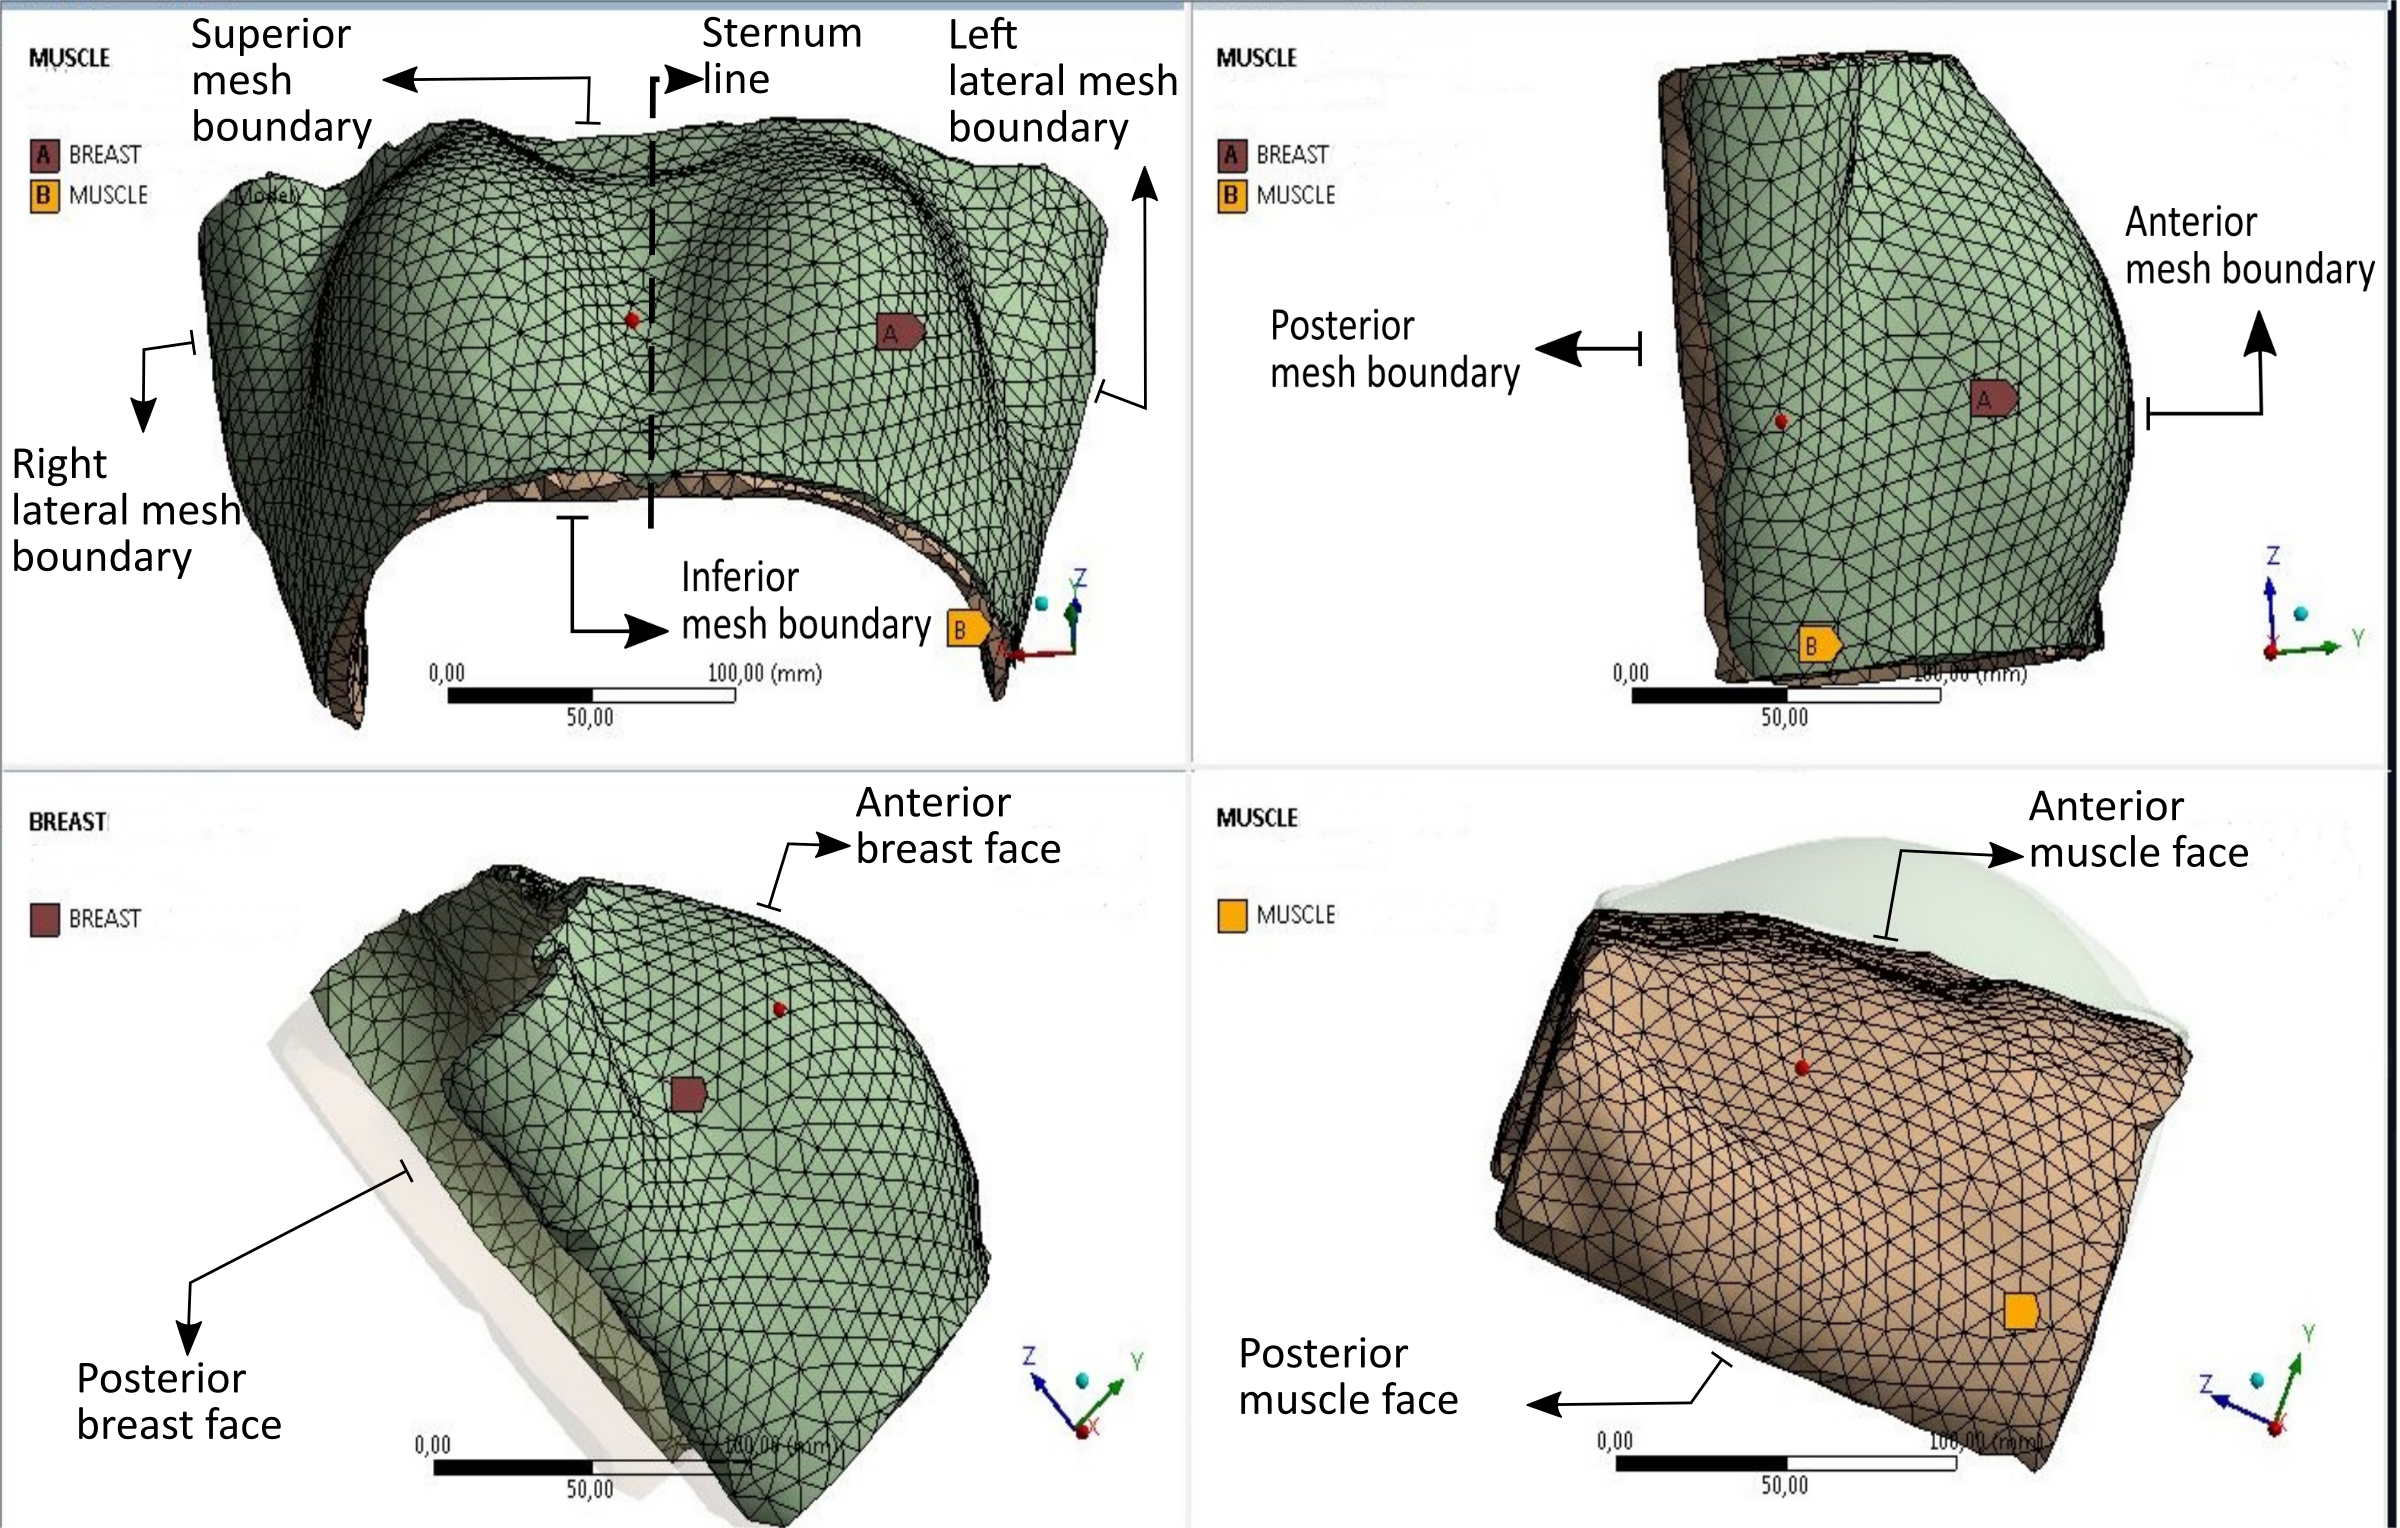
\includegraphics[width=0.9\textwidth,keepaspectratio]{figures/mesh_parts_2.png} 
\caption{Finite elements mesh boundaries}\label{fig:meshboundaries}
\end{figure}

Previous works have proved that to model breast deformation from prone to supine configurations breast tissues sliding over the chest wall have to be considered \citep{carter_application_2012,han_nonlinear_2014}. Moreover, anatomical books \citep{mugea2014aesthetic,clemente2011anatomy},  describe that the breast soft tissues are firmly attached to the deep fascia via suspensory ligaments but move freely over the pectoralis muscle.  Therefore, the juncture surface is modeled as a no-separation contact with a frictional behavior proposed by ANSYS Contact Technologies (see sec.\ref{subsection:surfaceinteractionmodels}). Penalty algorithm  is used with a meticulous control of contact normal and opening stiffness parameters. Stiffness parameters don't have a physical meaning and have to be identified by \textit{trial and error} methods. Because they are extremely sensitive to the underlying elements stiffness and to the local deformation direction, new values have to be identified for each new simulation case.    

To study the impact of the frictional coefficient parameter on tissues sliding, several simulation have been performed at different values of $\mu_f$. We found that, with the Coulombus friction law, even for a high values of $\mu_f$ the tissues sliding is overestimated. When simulating prone breast configuration from the supine one, the sliding overestimation results also in an unconvergent solution due to element distortion. At the contact surface, because of excessive sliding, the tissues accumulation in the region of the sternum line results in a sinuous surface  (fig. \ref{fig:overslidingProblem}) ; the finite elements  undergo important distortion and the solution is compromised. Therefore different strategies based on anatomical breast structures were investigated to limit the amount of sliding and to overcome solution instabilities (Annex 2). However, a small amount of friction improve the solution convergence capabilities (refer ansys manual), thus the friction coefficient is kept to $\mu_f = 0.1$. 
\begin{figure}[!h]
\centering
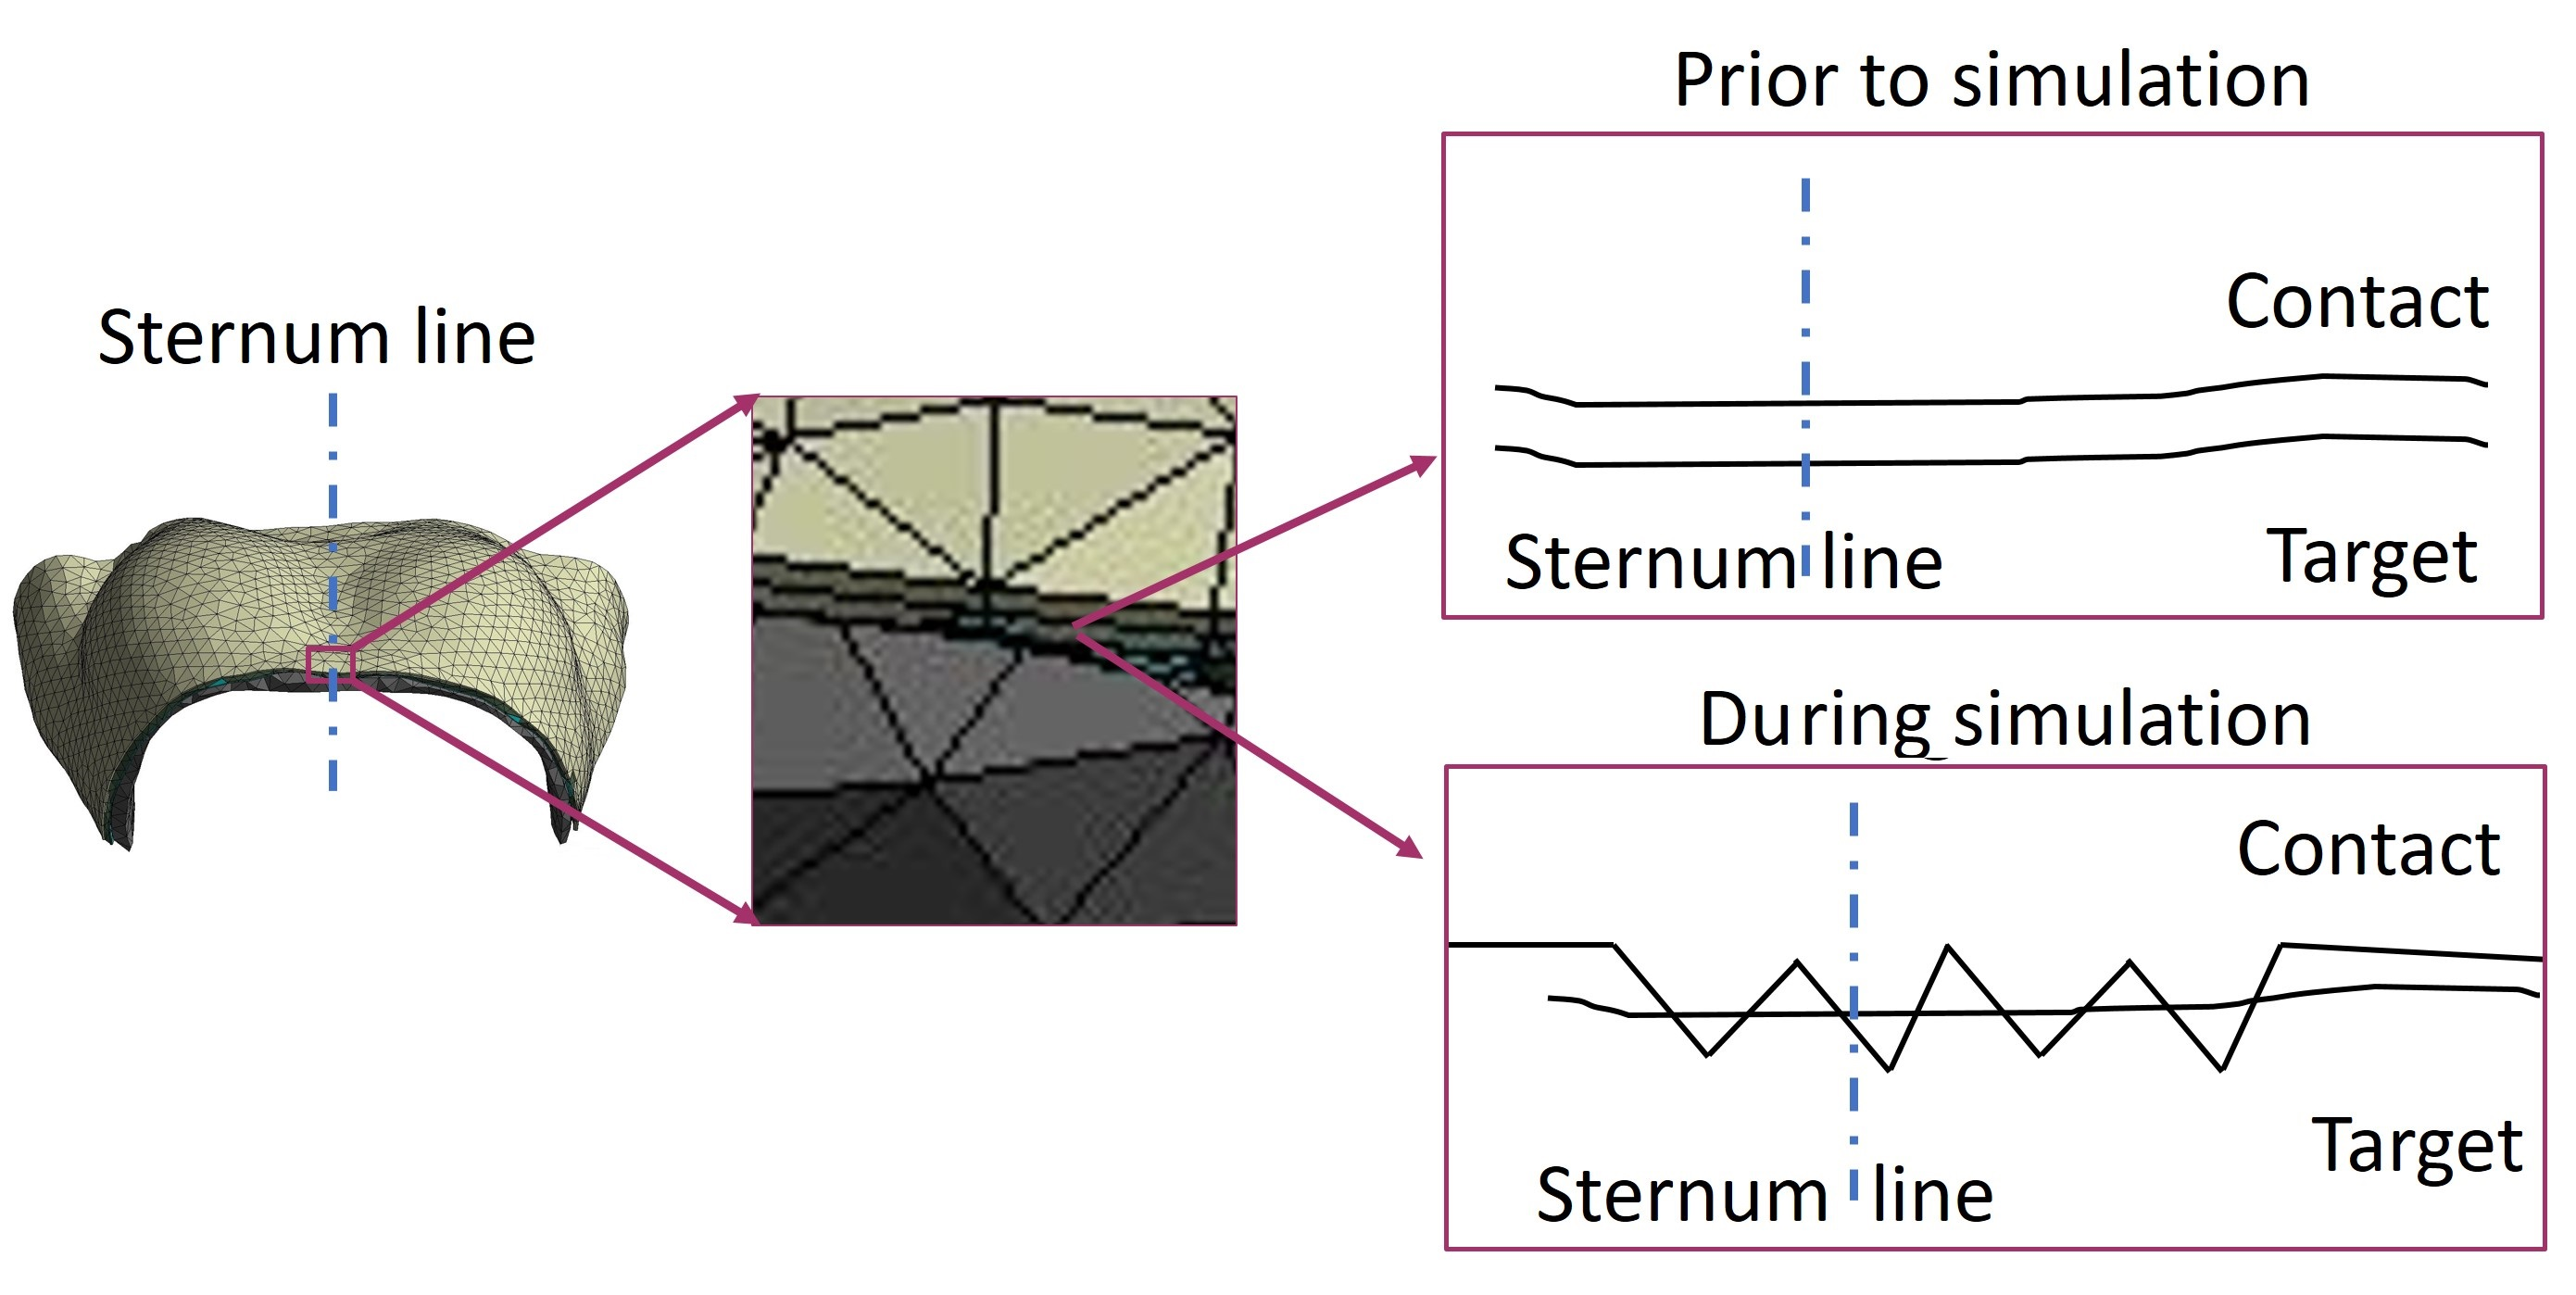
\includegraphics[width=0.7\textwidth,keepaspectratio]{figures/overslidingProblem.jpg} 
\caption{Tissues acumulation on the sternum line with excessive sliding}\label{fig:overslidingProblem}
\end{figure}
 
The selected  strategies chosen to control the amount of tissues sliding relies on ligamentous breast structures described on section \ref{subsection:internalstructures}. From breast support matrix only the largest structures are modeled, i.e. fascias and suspensory ligaments.  Superficial layer of superficial fascia is integrated in the skin layer, assuming a higher material stiffness. In addition, a new layer of 0.1mm thick shell elements is added at the juncture surface between muscle and breast tissue to model the deep layer of the superficial fascia. Shell elements and the underlying breast elements are sharing the same nodes. Since the deep fascia and muscle tissues are supposed to present similar elastic properties, the deep fascia is not explicitly modeled. Two ligamentous structures (inframammary ligament and deep medial ligament) are modeled using Ansys link type elements connecting breast posterior surface nodes to anterior muscle surface nodes (Figure \ref{fig:mesh_components_BC}).  


Several additional Dirichlet conditions are set on the mesh boundaries: superior and inferior ends of the deep fascia layer are constrained in Z direction; superior and inferior ends of skin layer are constrained in Y direction. For left and right lateral breast boundaries (Figure \ref{fig:meshboundaries}), Dirichlet conditions are too strong and preclude breast tissue to slide laterally. Therefore, in these regions new ligamentous structures are included with a cable-like behavior (fig. \ref{fig:mesh_components_BC}).



\begin{figure}[!h]
\centering
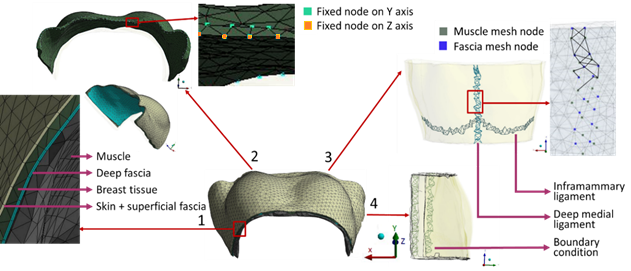
\includegraphics[width=0.9\textwidth,keepaspectratio]{figures/mesh_components.png} 
\caption{Components of the finite elements mesh.}\label{fig:mesh_components_BC}
\end{figure}

 The deep layer of superficial fascia is much stiffer than underlying adipose tissues. Due to imposed boundary conditions, the amount of sliding depends fascia's elasticity. The suspensory ligaments define regions were the breast sliding is minimal regardless of applied deformation. These additional stiff structure reduce the tissues sliding and improve the solution convergence capability. 

\section{Materials constitutive models}
\label{section:myConstitutivModels}

The final model consists of 6 types of tissues, wherein 4 tissues (glandular, fatty, muscle and skin ) are well described and regularly used for biomechanical modeling and 2 of them (fascia and suspension ligaments) with limited use and poorly described in literature. A large range of constitutive parameters are available for each tissue, however because of an  inconsistent interindividual variability, patient specific parameters have to be identified.  


 Here, all materials except the suspensory ligaments are modeled using the Neo-Hookean potential function. Breast ligaments are considered as linear materials.  Subject specific mechanical tissue properties are computed using an optimization process based on a multi-gravity loading simulation procedure (Figure \ref{fig:optimizationalgo}). First, for a given set of parameters $(E_{breast}$\nomenclature{$E_{xx}$}{Youngs's moduli of the material $xx$},$ E_{muscle}, E_{skin}, E_{fascia}, E_{ligam}$, $\nu$ \nomenclature{$\nu$}{Poisson's ratio}) the breast stress-free configuration is estimated by minimizing the difference between the simulated and measured breast geometry in prone configuration. Then, from the new estimated stress-free geometry, the supine breast configuration is derived. The estimated supine geometry is compared to the measured one using modified Hausdorff distance, thus representing the estimation error .  To avoid taking in account the geometry dissimilarity due to arms position, the modified Hausdorff distance is computed only on breast skin surface.  
The process implies multiple simulation based on imposed nodes displacement, therefore the FE mesh can be significantly altered before reaching an optimal stress-free geometry. Mainly for that reason we chose to perform an exhaustive manual rather than an automatic research of the optimal set of constitutive parameters. 


\begin{figure}[!h]
\centering
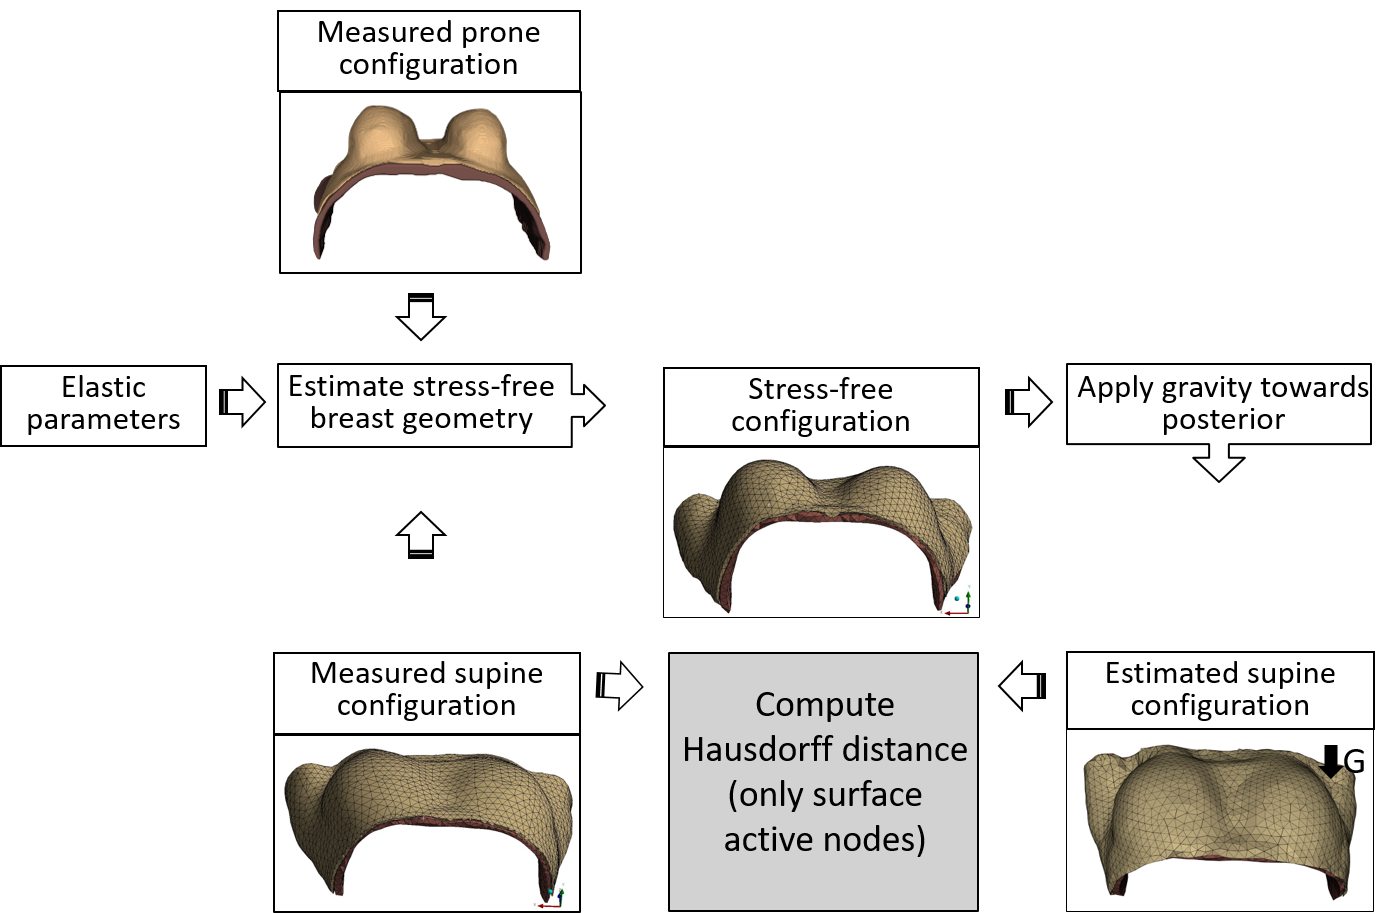
\includegraphics[width=0.9\textwidth,keepaspectratio]{figures/optimizationMaterialParameters.png} 
\caption{Process to estimate optimal material parameters}\label{fig:optimizationalgo}
\end{figure}
 
 An optimization process including finite elements simulation with 6 parameters results is a complex and time consuming problem. The model simplification is then performed in two steps. First, the parameters which variation have non-significant effect on simulation results are identified and set to a optimal fixed value. Next for parameters which variation have a high impact a sensitivity study is performed to redefine the search intervals and interval's discretization step.
 
 \subsection{Model simplification}

The breast tissues are mainly composed of water, an usual assumption  is to consider them as nearly incompressible materials \citep{fung_biomechanics_2013}. However,
previous works proposed a Poisson's ratio value ranging between $\nu = 0.3$ \citep{hopp_automatic_2013} and $\nu = 0.5$ \citep{gamage_modelling_2012}. In a multi-loading gravity simulation, the breast volume is nearly constant, thus, the influence of  Poisson's ratio on nodes displacements is studied only for values laying between $\nu = [0.45 , 0.495]$ (fig. \ref{fig:poissonRatio}). 

\begin{figure}[!h]
\centering
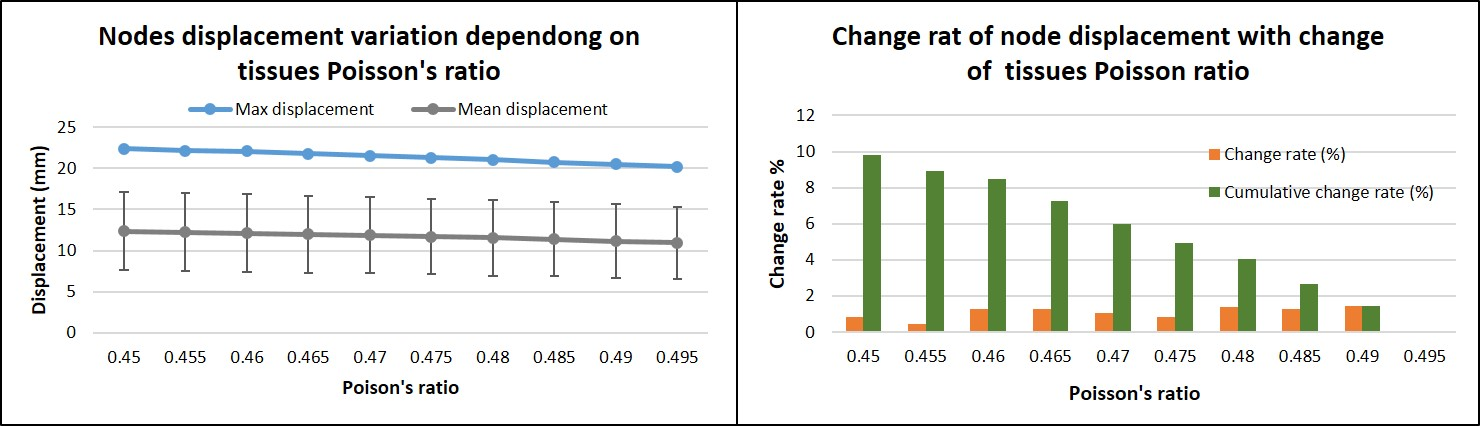
\includegraphics[width=0.9\textwidth,keepaspectratio]{figures/poissonRatio.jpg} 
\caption{Process to estimate optimal material parameters}\label{fig:poissonRatio}
\end{figure}

The simulations were performed by applying the gravity force in posterio-anterior direction on breast geometry from supine configuration. On the right hand side, the mean and the maximal displacement of the skin nodes is given for each values of $\nu$. On the left hand side the maximal difference of nodal displacement between two consecutive simulations (change rate) and and the maximal difference of node displacement between the actual and the less deformed geometry (cumulative change rate) are plotted. The change rate is computed within the assumption that the maximal displacement over the simulations set represents 100\% change rate. Non significant variations are observed on the mean and maximal displacement of skin nodes, thus a constant values of $\nu = 0.49$ was chosen.


The pectoral muscle together with the thoracic cage are the breast tissues support,under gravity loading the muscle deformation is neglected. Therefore, its Young's modulus was not included on the parametric study and was chosen large enough so that only minimal deformations occur ($E_{muscle}=10kPa$).

The  ligamentous breast structures are added with a cable-like behavior to reduce tissues sliding. Their young's modulus is also not included in the optimization process and is set sufficiently high ($E_{ligam}=500kPa$) to preclude their elastic deformation. 

The adipose and glandular tissues are known to be extremily soft and to undego large deformation under gravity loading.  \cite{calvo_polynomial_2015} proposed a uniform polynomial material model for the mixture of adipose and glandular tissues. The authors also shown that the breast outer shape deformation does not depend on glandular distribution but is highly dependent on its volumetric ratio. Here, the glandular and fatty tissues are also modeled as a single homogeneous material with an equivalent Young's modulus $E_{breast }$. The mechanical properties of the equivalent breast tissue is in direct relation with glandular and adipose volumes ratios. Because the left and right breasts may have a different granularity, two different parameters are considered ($E_{breast}^l$ \nomenclature{$E_{xx}^{l/r}$}{Young's modulus of the material xx for the left/right breast}, $E_{breast}^r$).

Breast skin and superficial fascia are an essential part of the breast support matrix. The two layers are much stiffer than breast tissues and are the structures governing the amount of deformation. Their elastic behavior was included on the optimization process.

 Based on existing publications, an interval of possible values are given in table \ref{table:minandmaxelasticmodulus} for each parameter included in the optimization process $(E_{breast}^l$, $E_{breast}^l$, $E_{skin}$, $E_{fascia})$. To characterize model sensitivity to parameters variations, a set of simulation were performed. The defined interval was discretized by steps of 10\% and at each step the skin node displacement was computed. Results of the corresponding simulations are shown on fig.\ref{fig:materialPropDiscretization}. As previously, the first column represents  the variation of mean and maximal displacement of skin nodes in function of the elastic parameter of each material; the second column represent the change rate and the cumulative change rate of skin nodes displacement.


\begin{table}[!h]
\centering
\begin{tabular}{|c||c|c|c||c|c|c|}
\hline
&\multicolumn{3}{|c||}{Search intervals}& \multicolumn{3}{c|}{Search intervals}\\
&\multicolumn{3}{|c||}{ from bibliographic data}& \multicolumn{3}{c|}{ after model simplification}\\
\hline
\hline
& Breast & Skin & Fascia & Breast & Skin & Fascia \\
\hline
Min (kPa)  & 0.3 & 7.4 & 100 & 0.3 & 2 & 50\\
\hline
Max (kPa) & 6 & 58.4 & 5000& 4& 20 &250 \\
\hline
\end{tabular}
\caption{Minimal and maximal value (in kPa) for Young’s modulus.}
\label{table:minandmaxelasticmodulus}
\end{table}

The figure shows that the model is very sensitive to the variation of Young’s modulus of breast tissue, skin and fascia (Figure \ref{fig:materialPropDiscretization}). However, beyond some values, the materials become too stiff and do not change significatively under gravity loadings.  Therefore, the search intervals for breast tissue and skin Young’s modulus are reduced such that a larger value impacts the cumulative change rate less than 20\% (max displacement less than $\sim 5mm$). As the fascia stiffness governs the lateral displacement and shows a smaller variation over the search interval, a threshold of 10 \% ($\sim 2.5mm)$ is chosen. The obtained results are summarized in table \ref{table:minandmaxelasticmodulus} 

\begin{figure}[!h]
\centering
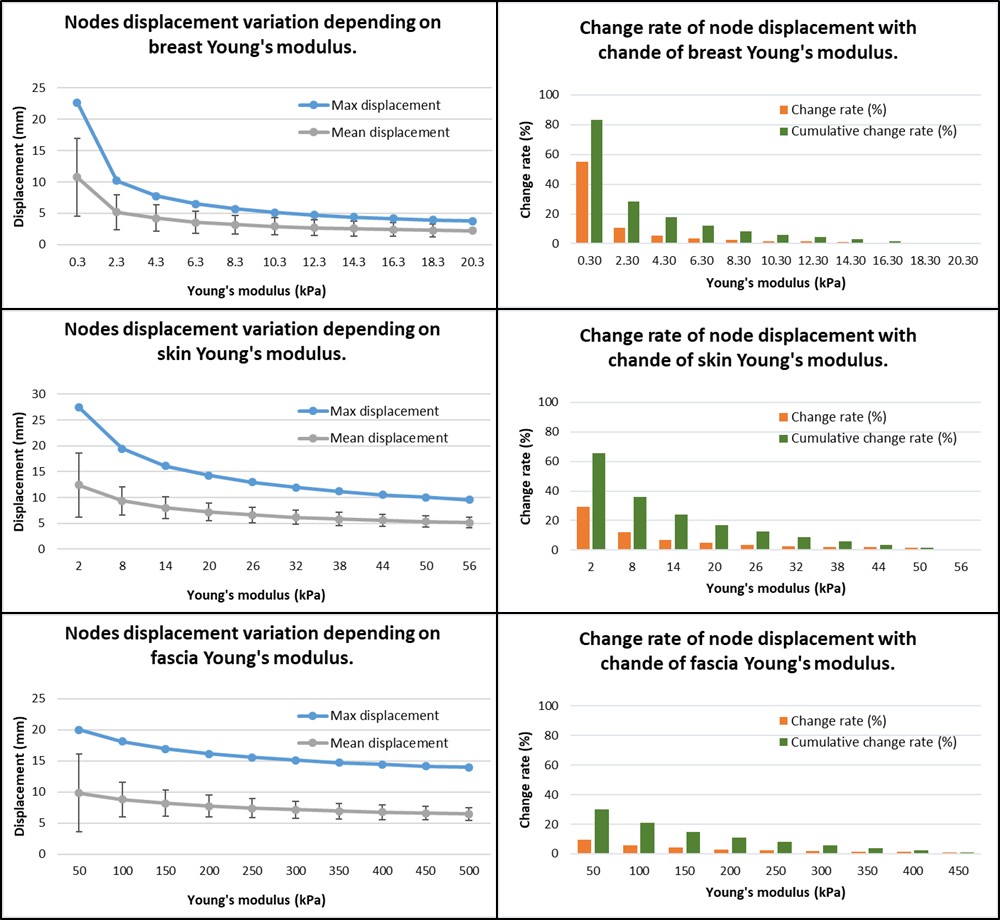
\includegraphics[width=0.9\textwidth,keepaspectratio]{figures/materialPropDiscretization.png} 
\caption{First column: relation between maximal and mean nodes displacement and the equivalent Young's modulus variation for different tissues. Second column: rate and cumulative change rate of node displacement in function of quivalent Young's modulus}\label{fig:materialPropDiscretization}
\end{figure}

\subsection{Estimation of optimal constitutive parameters}
To perform the optimization process, the new intervals defined by sensitive analysis are discretized by steps of $0.1 kPa$, $1kPa$ and $40 kPa$. The discretization step are chosen such that the change rate between two consecutive simulations is less than 10\%.

The previously described multi-loading gravity process was performed for each parameters set and the model error distribution is shown in fig \ref{fig:optimizationresults}. The contour lines are estimated by linear interpolation between two consecutive succeeded simulations. We found that the breast tissues Young's modulus is lower than the ones proposed in the bibliography, therefore more simulations were done outside the defined interval. However, for very low values, below 0.2 kPa, 2 kPa and 80 kPa for breast, skin and fascia's Young's moduli respectively, the tissues deformation is too large and the finite element mesh becomes degenerated at the first step of multi-loading simulation. For values above 1 kPa, 5 kPa and 160 kPa, tissues deformation is too small compared to the ones measured on the MR images and the simulations were excluded. All other missing values correspond to failed simulations due to a non-converging force, specifically in the region of the contact surface between the breast and the muscle.

\begin{figure}[!h]
\centering
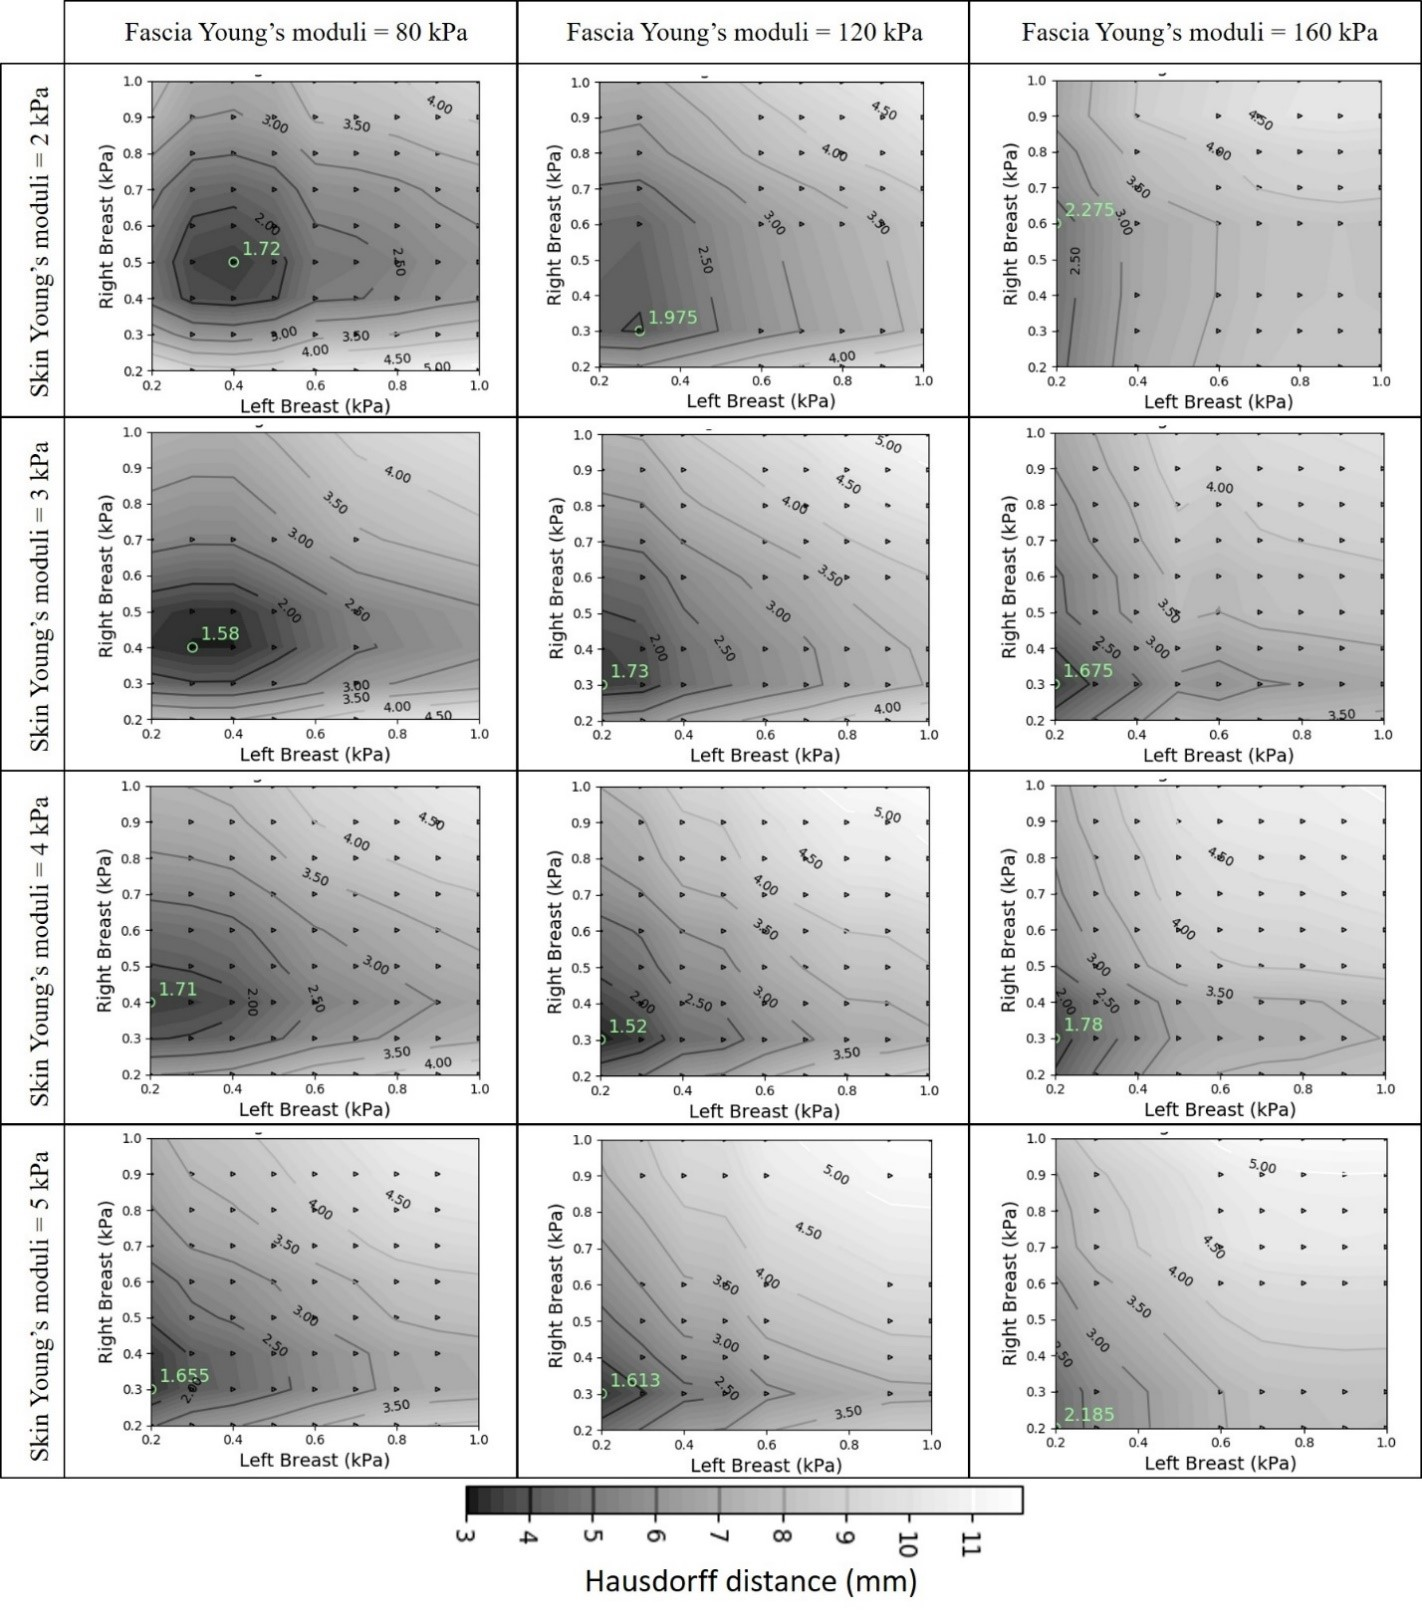
\includegraphics[width=0.9\textwidth,keepaspectratio]{figures/optimizationMaterialParameters2.png} 
\caption{Hausdorff distance on the skin surface over the constitutive parameters space}\label{fig:optimizationresults}
\end{figure}

 

For very soft fascia ($E_{fascia} = 80kPa$), the lateral displacement of breast tissues is more important than the one measured on  MR images. Conversely, for stiff fascia material ($E_{fascia}=160 kPa$) the amount of sliding is too small; therefore, to match the breast geometry in supine configuration,very low values for Young modulus are required ( $E_{breast}< 0.2kPa$). For such low values, the breast tissues are highly deformed, thus the finite elements undergo distortions. Because of  errors in elements formulation the simulations giving the minimal Hausdorff distance have not succeed.   

The set of parameters giving the best match between simulated and measured supine breast configurations is ($E_{breast}^r=0.3 kPa$,$E_{breast}^l=0.2 kPa$,$E_{skin}=4 kPa$,$E_{fascia}=120 kPa$).  


\subsection{Conclusion}


This chapter propose a new biomechanical breast model. The model was build on patient-specific data extracted from MR images in different breast configurations. New structures as pectoral fascia and suspensory breast ligaments were considered and their impact on breast mechanics was analyzed in a multi-loading gravity simulations.  A particular attention was granted to the estimation of subject-specific breast stress-free geometry and tissues constitutive models.
 
The proposed breast model shows that introducing a sliding movement of the breast tissues over the pectoral muscle together with a ligamentous system and pectoral fascia, allows a better estimation of supine and prone configurations. The latter support structures provide a finer method for boundary conditions definition which also improve the convergence capability of the solution. It can be stated that the obtained Young’s modulus of breast soft tissues is relatively low (0.2-0.3kPa for breast tissues and 4kPa for skin), which is a contradictory result compared to some studies on the field. However, only with such small values together with sliding boundary conditions that prone and supine configurations were accurately estimated.

With the obtained optimal constitutive parameters set  ($E_{breast}^r=0.3 kPa$,$E_{breast}^l=0.2 kPa$,$E_{skin}=4 kPa$,$E_{fascia}=120 kPa$) and the corresponding  breast stress-free configuration simulations with the gravity force oriented in different directions could by simulated. The next chapter evaluate the model accuracy on three breast configurations: supine, prone and supine tilted.
   



